\documentclass{article}
\usepackage{graphicx} % Required for inserting images
\usepackage{todonotes}
\usepackage{amsmath}
\usepackage{easyReview}
\usepackage{amssymb}
\usepackage{amsfonts}
\usepackage{algorithm}
\usepackage{booktabs}
\usepackage{array}
\usepackage{cite}
\usepackage{algpseudocode}
\usepackage{float}
\usepackage[]{geometry}
\usepackage{todonotes}
\usepackage[T1]{fontenc}

% Decreasing the margins for readability
\geometry{
	left=1in,    % Left margin
	right=1in,   % Right margin
	top=1in,     % Top margin
	bottom=1in   % Bottom margin
}


\title{CUDA-sDBSCAN: GPU Accelerated Density Based Clustering With Random Projections}
\author{   
    Hugo Phibbs % TODO add complete affiliations, emails etc.
}
\date{March 2024} % TODO change for publication

% Marcos
\newcommand{\br}{\mathbf{r}}
\newcommand{\bq}{\mathbf{q}}
\newcommand{\bx}{\mathbf{x}}
\newcommand{\eps}{\epsilon}
\newcommand{\Bq}{B_{\eps}(\bq)}
\newcommand{\Bx}{\widetilde{B}_{\eps}(\bx)}
\newcommand{\Bqt}{\widetilde{B}_{\eps}(\bq)}
\newcommand{\Sd} {\mathcal{S}^{d-1}}
\newcommand{\Nqt}{\widetilde{N}(\bq)}
\newcommand{\bu}{\mathbf{u}}
\newcommand{\bv}{\mathbf{v}}
\newcommand{\bw}{\mathbf{w}}
\newcommand{\bR}{\mathbf{R}}
\newcommand{\bX}{\mathbf{X}}
\newcommand{\bP}{\mathbf{P}}


\begin{document}

\maketitle

\begin{abstract}
    
\end{abstract}

\section{Introduction}	
DBSCAN \cite{DB_SCAN_1996} is density based clustering based algorithm with many applications in areas such as machine learning, data mining and biology \cite{campello_density-based_2020}. It's applicability has stood the test of time - appearing in a plethora of data analysis tools such as ELKI, scikit-learn, R and Weka.

% TODO can add more here as time progresses.

\section{Related Work}

There have been a myriad of research in the past to adapt DBSCAN for large scale datasets. These attempts can be broadly classified into the usage of data indexing, approximating clusters, specialised hardware and distributed computing.

Work to scale up DBSCAN with data indexing \cite{ohadi_sw_dbscan_2020, huang_grit-dbscan_2022} \comment{}{why are these refs not showing up?} can be effective at increasing the \comment{scalability of DBSCAN}{reference for this}. Although they have shown to be successful for low dimensional datasets, they are ill-suited to large scale applications because of run-off effects with the complexity of effectively indexing high dimensional data. 

Research to approximate DBSCAN \cite{S_DBSCAN, schneider_scalable_2017, jiang_faster_2020} has also proved effective at scaling DBSCAN. Sampling approaches such as K-DBSCAN \cite{gholizadeh_k-dbscan_2021} and sngDBSCAN \cite{jiang_faster_2020} \comment{are potentially efficient, except they can rely on the a wise choice of sampling parameters - which can be difficult.}{feel like more can be said here}

Due to the parallelizable nature of DBSCAN, other approaches \cite{andrade_g-dbscan_2013, poudel_cuda-dclust_2021, thapa_memory-efficient_2010} have focused on using a GPU to accelerate DBSCAN. CUDA-DClust+ \cite{poudel_cuda-dclust_2021} utilizes a tree indexing structure as-well as a GPU to accelerate computation. While it is excellent for applications with small scale data-sets, it is limited to this use case due to complexity of creating an indexing tree over large dimensions. Andrade et al's G-DBSCAN \cite{andrade_g-dbscan_2013} focuses on using graph principles along with a GPU to scale DBSCAN. However, due to it's usage of an graph adjacency list, G-DBSCAN can prove to be severely memory intensive \cite{mustafa_experimental_2019}. \comment{There is also little experimental data to support the usage of G-DBSCAN dimensions greater than 2. }{honestly, not too sure about this! - its a claim made in CUDA-DClust+ paper - end of p40}

% TODO add more here, not sure. Just looks a little light right now.

\section{Preliminaries}

\subsection{DBSCAN}
\comment{}{Perhaps comment that the below is a naive implementation of DBSCAN?}
In a nutshell, DBSCAN \cite{DBSCAN} is an algorithm to cluster related data points together based on a given distance metric between points. The algorithm is composed of two key processes: the classification of points identified as \textit{core} and the formation of clusters based on these \textit{core} points.

For the sake of explanation consider a set of data points $X = \{\bx_1, \bx_2, \dots, \bx_n\}$, where $\textit{dim}(\bx_i) = d$. The identification of core points can be completed as follows:

\begin{enumerate}
	\item For each data point $q \in X$ find the distance  $\textit{dist}(\bx, \bq)$  to all other data points $\bx \in X$. If $\textit{dist}(\bx, \bq)$ is less than the maximum clustering distance $\eps$, add $\bx$ to the neighbourhood set of $\bq$, denoted by $\Bq$ 
	\item For each $\bq \in X$, if $|\Bq|$ is greater than or equal to a threshold $minPts$,then the point $\bq$ is a \textit{core point}. Add the tuple $(\bq, \Bq)$ to the core point set $C$. 
\end{enumerate}

The pseudo code for the identification of key points is shown in algorithm \ref{alg:dbscan-core-points}.

% Need to add citations for these?
\begin{algorithm}[H]
	\caption{DBSCAN, classification of core points}
	\label{alg:dbscan-core-points}
	\begin{algorithmic}[1]
		\State \textbf{Input:} Data points $X = \{\bx_1, \bx_2, \dots, \bx_n\}$, $\eps$, $minPts$
		\State \textbf{Output:} Set containing core points and their $\eps$-neighbourhoods
		
		\State Initialize $C = \emptyset$
	
		\For{each data point $\bq \in X$}
		\State Initialize $\Bq = \emptyset$
		\For{each data point $\bx \in X$}
		\State Compute $\textit{dist}(\bx, \bq)$
		\If{$\textit{dist}(\bx, \bq) < \eps$}
		\State Add $\bx$ to $\Bq$
		\EndIf
		\EndFor
		\If{$|\Bq| \geq minPts$}
		\State Add $(\bq, \Bq)$ to $C$
		\EndIf
		\EndFor
		
	\end{algorithmic}
\end{algorithm}

Once core points are identified, the data set can be partitioned into clusters. A cluster is formed by considering all points that are within \textit{direct} or \textit{transitive} $\eps$ distance from each other. Given the identification of core points and their neighbourhoods, clusters can be formed using algorithm \ref{alg:dbscan}. The result of the DBSCAN algorithm is a graph $G$, where each connected component is a cluster of the data set $X$

% TODO ok that I literally copy pasted this from sDBSCAN source?
\begin{algorithm}[H]
	\caption{DBSCAN, forming clusters}
	\label{alg:dbscan}
	\begin{algorithmic}[1] % [1] for line numbers
		\State \textbf{Inputs}: $X, \eps, minPts$ the set $C = \{ (\bq, \Bq) \, | \, \bq \text{ is core} \}$
		\State $G \gets$ initialize empty graph
		\For {each $\bq \in C$}
		\State Add an edge (and possibly a vertex or vertices) in $G$ from $\bq$ to all \textit{core} points in $\Bq$
		\State Add an edge (and possibly a vertex) in $G$ from $\bq$ to \textit{non-core} points $\bx \in \Bq$ if $\bx$ is not connected
		\EndFor
		\State \textbf{return} connected components of $G$
	\end{algorithmic}
\end{algorithm}
% TODO, how to change the above, such that the set C initialization is more neat?

Once the clustering step is complete, we can classify points into several type - these are described in the list below. Figure \ref{fig:core-points} details this concept further.

\begin{enumerate}
	\item \textbf{Core Points} these are points with at-least $minPts$ points within $\eps$ distance of itself.
	\item \textbf{Border Points} these are \textit{non-core} points that are nevertheless included into a given cluster.
	\item \textbf{Noise Points} these are points that are \textit{neither} core or border points. They are not included in any clusters.
\end{enumerate}

% TODO replace with the actual fig, this was simply a screen snip
\begin{figure}[H]
	\centering
	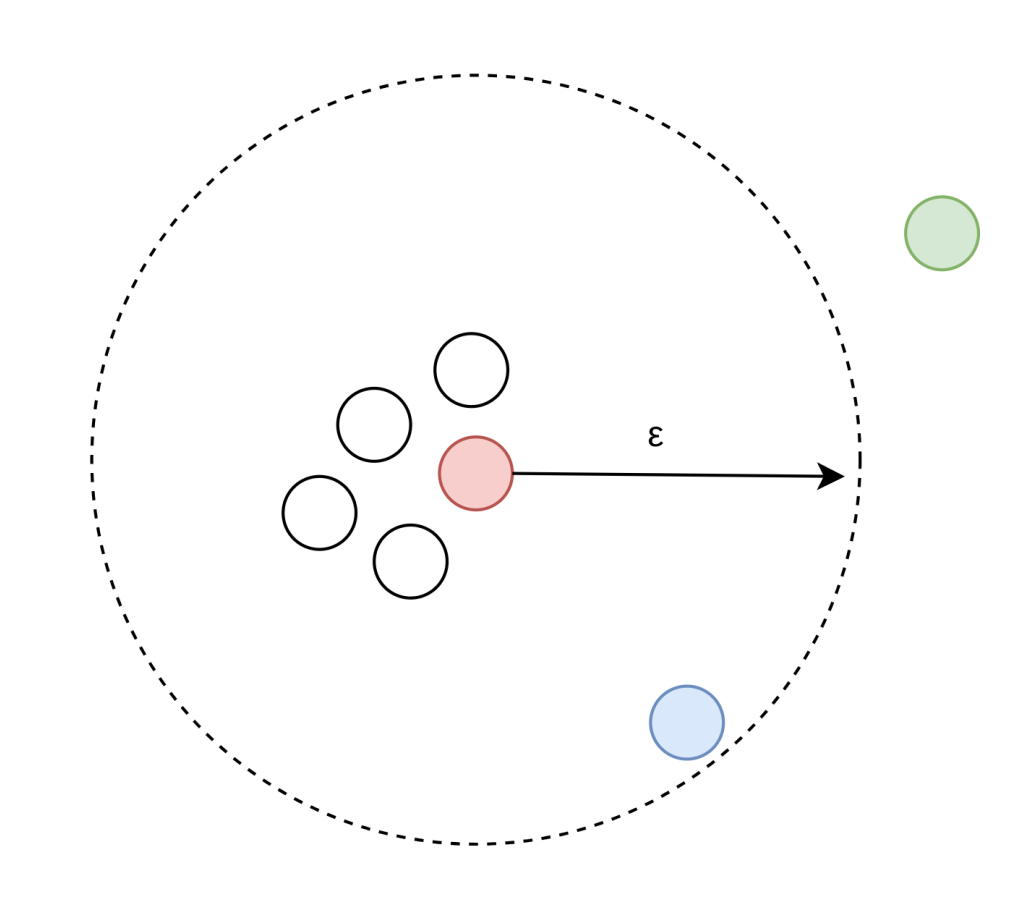
\includegraphics[width=0.5\linewidth]{figs/core_points.png}
	\caption{Classification of Core Points \cite{S_DBSCAN}}
	\label{fig:core-points}
\end{figure}

Figure \ref{fig:clusters} shows an example of created clusters from DBSCAN. The red points are identified as core, the blue as noise, and the yellow border points. 

\begin{figure}[H]
	\centering
	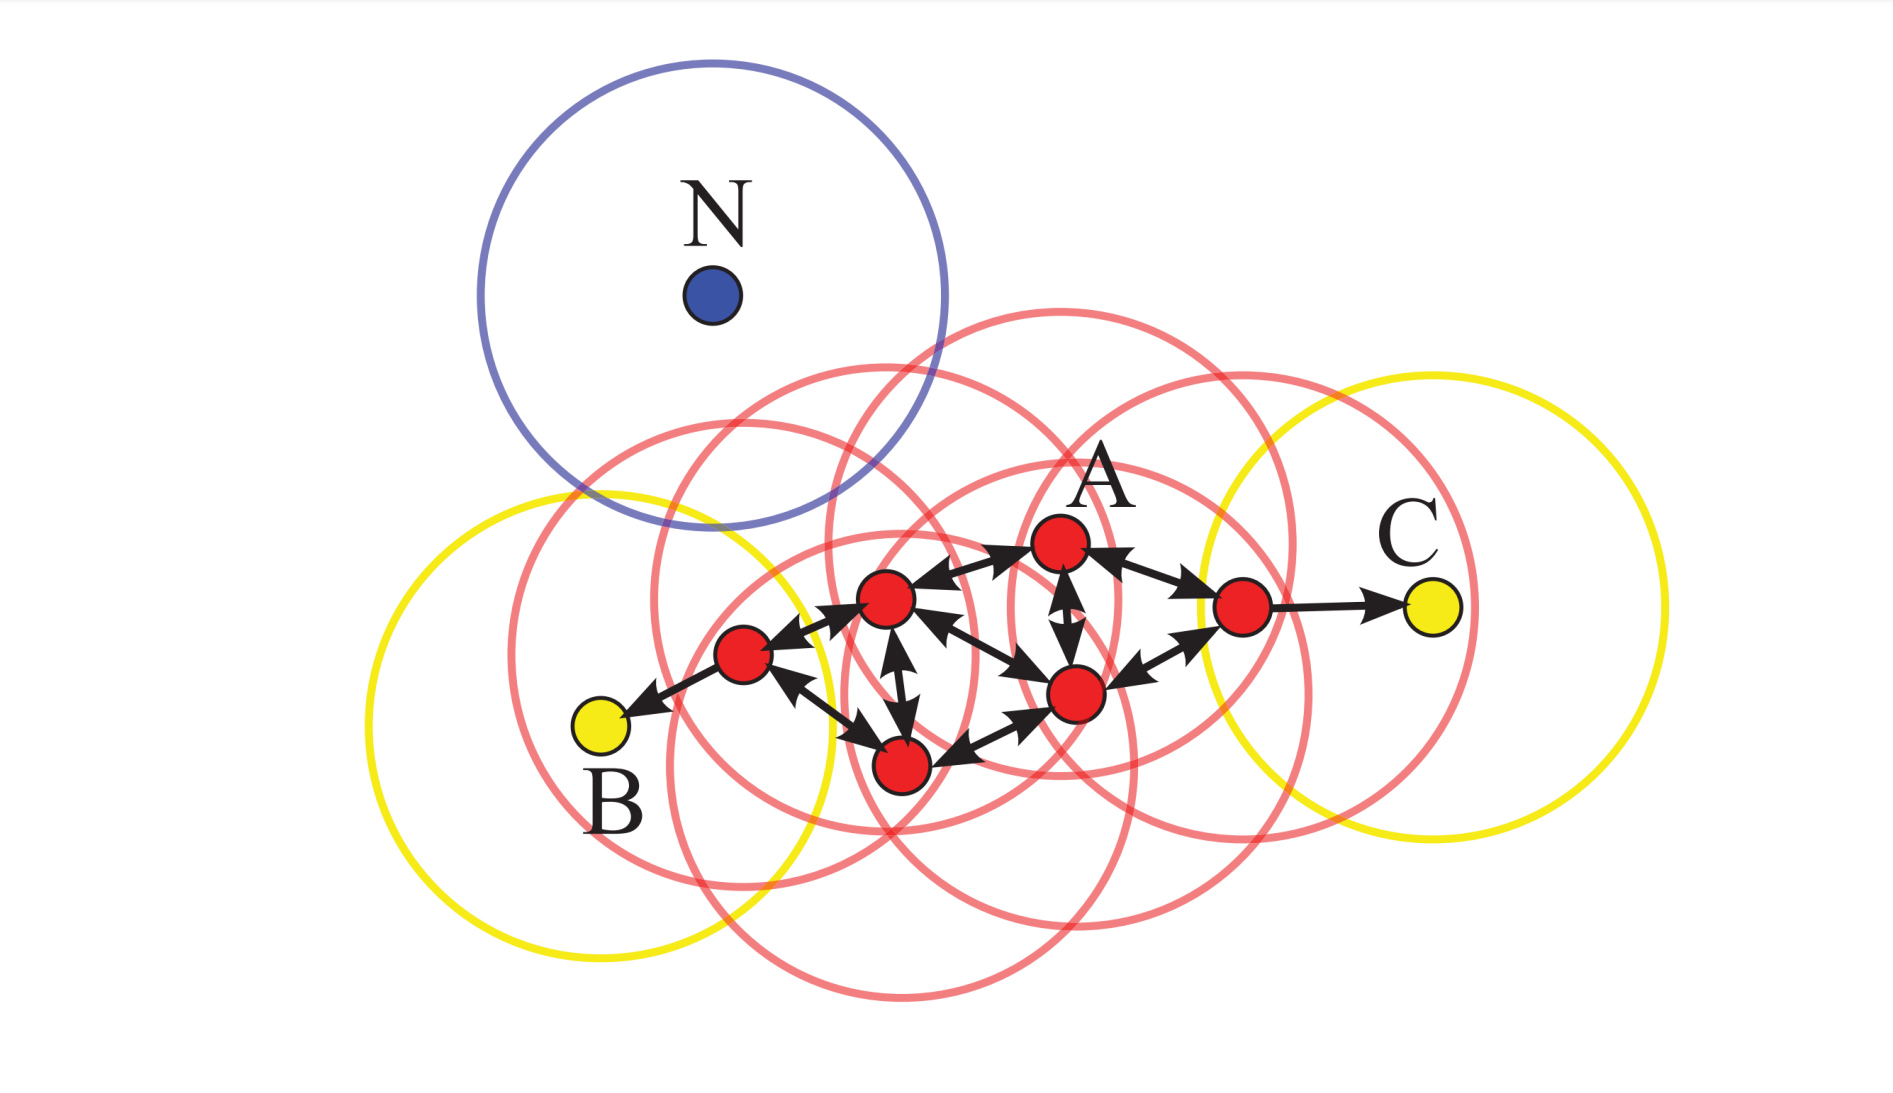
\includegraphics[width=0.5\linewidth]{figs/formation_of_clusters.png}
	\caption{The formation of clusters from DBSCAN \cite{DBSCAN_REVISITED}}
	\label{fig:clusters}
\end{figure}

% TODO replace with the actual fig, this was simply a screen snip
\todo{Add a comment on different distance metrics that can be used}

\subsection{sDBSCAN}
\comment{}{Comment here about the scalability of DBSCAN, and how this is addressed with sDBSCAN.}
sDBSCAN\cite{S_DBSCAN} is an implementation of DBSCAN based on using random projections to rapidly speed up the $\eps$-neighbourhood search for each particular data point. Besides the given DBSCAN inputs of $X$, $\eps$, and $minPts$, sDBSCAN adds a few more parameters - these are described in table \ref{tab:definitions}.

\begin{table}[H]
	\centering
	\begin{tabular}{|>{\raggedright}p{0.15\linewidth}|>{\raggedright\arraybackslash}p{0.7\linewidth}|}
		\hline
		\textbf{Parameter} & \textbf{Description} \\ 
		\hline
		$\mathbf{Y}$ & A set of $D$ random vectors with the same dimension as points in $X$. Each random vector has coordinates sampled from the standard normal distribution. Formally: $\mathbf{Y} = \left\{ \br^i \mid \br^i \in \mathbb{R}^d, \ \br^i \sim \mathcal{N}(0,1), \ i \in [D] \right\}$ \\ \hline
		$k$ & The number of closest/furthest random vectors from $Y$ to store for each query point $\bq \in X$ \\ \hline
		$m$ & The number of closest/furthest query points from $X$ to store for each random vector $\br \in Y$. Where $m > minPts$.\\ \hline
	\end{tabular}
	\caption{Definitions and descriptions of sDBSCAN's parameters}
	\label{tab:definitions}
\end{table}

\comment{}{Perhaps some more extrapolation on the usage of the random points, before going straight into the business of projections}

The sDBSCAN algorithm can be summarised into a few key steps: pre-processing, identification of key points, and formation of clusters. The pre-processing steps are as follows:

\begin{enumerate}
	\item For each random vector $\br_i \in Y$, calculate it's projection to each query point $\bq \in X$. 
	\item For each query point $\bq \in X$, using the projections store its top $k$ closest and furthest random vectors. The set of points 
	\item For each random vector $\br_i \in Y$, using the projections, store its top $m$ closest and furthest data set points.
\end{enumerate}

Once preprocessing is complete, we can define the \textit{Candidate Neighbourhood Set} $\Nqt$ of a given query point $\bq$. This set is composed of the $2km$ vectors that are either the $m$ closest points to the closest $k$ random vectors to $\bq$, or the $m$ furthest points to the $k$ furthest random vectors to $\bq$. $\Nqt$ is essentially the set of points that is searched when forming the approximate $\eps$-neighbourhood set $\Bqt$ of a query point $\bq$ - this will be clear after describing the complete sDBSCAN algorithm. 

Algorithm \ref{alg:preprocessing} shows the pseudo code for sDBSCAN's preprocessing steps.

\begin{algorithm}[H]
	\caption{Preprocessing}
	\label{alg:preprocessing}	
	\begin{algorithmic} [1]
		\State {\bf Inputs}: $X \subset \Sd$, $D$ random vectors $\br_i$, $k, m = O(minPts)$		
		%
		\State \textbf{for} each $\bq \in X$, compute and store top-$k$ \textcolor{blue}{nearest} and top-$k$ \textcolor{blue}{farthest} vectors $\br_i \in \mathbf{Y}$ to $\bq$.
		\State \textbf{for} each random vector $\br_i \in \mathbf{Y}$, compute and store top-$m$ \textcolor{blue}{nearest} and top-$m$ \textcolor{blue}{farthest} points to $\br_i$.		
		%
		\normalsize		
	\end{algorithmic}
\end{algorithm}

From here, the preprocessing steps are essentially used to guide an informed search for the $\eps$ neighbourhood of each data point $\bx \in X$. This step uses the random projections to form an approximate $\eps$-neighbourhood set $\Bqt$ for each data-set point $\bq$. The pseudo code for this step is shown in \ref{alg:neighborhood}. Once this step is complete, perform the standard DBSCAN clustering step \ref{alg:dbscan} on the set of estimated core points and their neighbourhoods sets $\Bqt$ for $\bq$ identified as core. The pseudo code for this step is shown in \ref{alg:sdbscan}

\begin{algorithm}[H]
	\caption{Finding core points and their neighborhoods}
	\label{alg:neighborhood} 									
	\begin{algorithmic} [1]
		\State {\bf Inputs}: $X \subset \Sd$, $\mathbf{Y}$, $k$, $\eps$, $m = O(minPts)$		
		%
		\State Initialize an empty set $\br_{\bq}$ for each $\bq \in X$
		% \State{{\color{red}\texttt{\#pragma omp parallel}}} \Comment{Multi-threading directive}
		\For{\text{each} $\bq \in X$}
		% \State {\br_{\bq} \gets \emptyset}
		\For{\text{each} $\br_i$ from top-$k$ \textcolor{blue}{nearest} random vectors of $\bq$}
		\For{\text{each} $\bx$ from top-$m$ \textcolor{blue}{nearest} points of $\br_i$}
		\If{$dist(\bx, \bq) \leq \eps$}
		\State Insert $\bx$ into $\widetilde{B}_\eps(\bq)$ and insert $\bq$ into $\Bx$
		\EndIf                        
		\EndFor                    
		\EndFor
		\For{\text{each} $\br_i $ from top-$k$ \textcolor{blue}{farthest} random vectors of $\bq$}
		\For{\text{each} $\bx$ from top-$m$ \textcolor{blue}{farthest} points of $\br_i$}
		\If{$dist(\bx, \bq) \leq \eps$}
		\State Insert $\bx$ into $\Bqt$ and insert $\bq$ into $\Bx$
		\EndIf                        
		\EndFor                    
		\EndFor
		\EndFor
		%
		% \State{{\color{red}\texttt{\#pragma omp parallel}}} \Comment{Multi-threading directive}
		\For{\text{each} $\bq \in X$}
		\If{$|\Bqt| \geq minPts$}
		\State Identify $\bq$ as the core point
		\State Store $\Bqt$ as an approximate result of $\Bq$
		\EndIf
		\EndFor            
		%
		\normalsize		
	\end{algorithmic}
\end{algorithm}


\begin{algorithm}[H]
	\caption{sDBSCAN}
	\label{alg:sdbscan} 									
	\begin{algorithmic} [1]
		\State {\bf Inputs}: $X \subset \Sd$, $Y$, $\eps$, $minPts$	
		%
		\State {Call Algorithm~\ref{alg:preprocessing} for preprocessing with $m = O(minPts)$}
		\State {Call Algorithm~\ref{alg:neighborhood} to find the set \newline $C = \{ (\bq, \Bqt) \, | \, \bq \text{ is identified as core} \}$}
		\State {Call DBSCAN (Alg.~\ref{alg:dbscan}) given the output $C$ from Algorithm~\ref{alg:neighborhood}}
		%
		\normalsize		
	\end{algorithmic}
\end{algorithm}

\subsection{GPU Programming with CUDA}

A GPU (Graphical Processing Unit) is based around the idea of having using hundreds to thousands of independent cores to complete tasks in a parallelised manner. This strategy excels in areas such as linear algebra, sorting, and differential equations \cite{Owens2008}. To ease the development of applications that utilize a GPU, NVIDIA, a major manufacturer of GPU chips, has created the CUDA Platform \cite{nvidia_cuda}.
For the purposes of this paper, we will look at the typical architecture of a NVIDIA GPU, then see how this relates to the programming model of CUDA.

% TODO ok to cite IGN?
A GPU is primarily split in two several \textit{streaming multi-processors} (SMs). An individual SM is composed of a multitude of \textit{streaming processors} (SPs), however, for ease of explanation, we can consider an SP to be equivalent in nomenclature to a \textit{CUDA Core}. A typical modern GPU contains 50-100 SMs and thousand of CUDA Cores, for example an RTX 4080 GPU contains 80 SMs and 10240 CUDA Cores \cite{IGN4080SuperReview}. For our purposes, a single CUDA Core can be considered the smallest unit of a GPU - it executes a unit of instruction called a \textit{thread}.

% TODO whats the diff between a streaming processor and a CUDA core?

\begin{figure}[H]
	\centering
	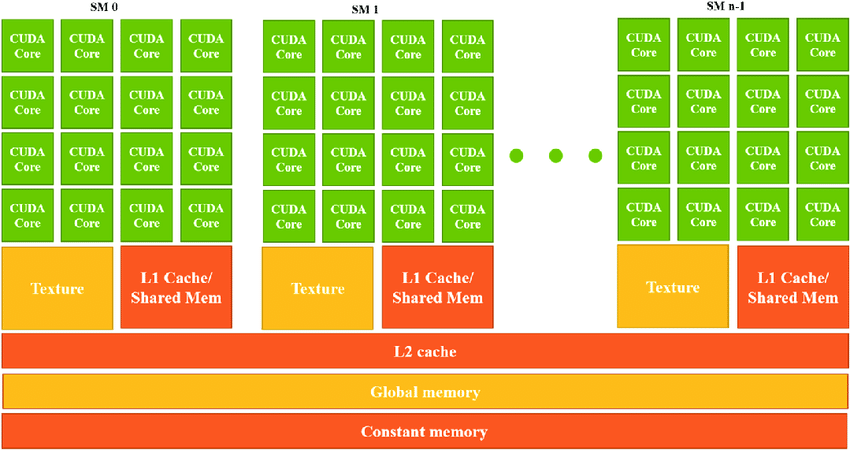
\includegraphics[width=0.7\linewidth]{figs/gpu-architecture.png}
	\caption{Simplified overview of typical GPU architecture \cite{GPUOptical}}
	\label{fig:gpu-architecture}
\end{figure}

For ease of development, the CUDA Platform abstracts the low level GPU hardware into a programming model with a \comment{few key concepts}{perhaps say why this is necessary}. At the highest level there is a \textit{kernel grid}, this executes a single set of instructions called a \textit{kernel} across a GPU. A
simple example of a kernel could be a function to add two vectors together. A grid is then sub-composed into \textit{thread blocks}, which in-turn contain \textit{threads}. Multiple thread blocks can be executed on a single SM, but an individual thread block cannot split it's execution across multiple SMs. A single thread executes one instance of a kernel on a CUDA Core. For a graphical representation of these concepts, see figure \ref{fig:nvidia-cuda-model}. Threads are executed in groups called \textit{warps}, which come in sizes of multiple of 32. To maximise occupancy of an SM while a block is being executed, the number of threads per block should be a \comment{multiple of 32}{find a reference for this}.


As an example of these concepts, take for instance the vector addition problem $\mathbf{u} + \mathbf{v} = \mathbf{w}$ where $dim(\mathbf{u}) = dim(\mathbf{v}) = 1048576$. One could launch a kernel-grid containing $1024$ blocks, with each block containing $1024$ threads. The single thread could be defined to simply perform the operation $\mathbf{u}[i] + \mathbf{v}[i] = \mathbf{w}[i]$ for a given index $i$. A potential kernel to use for this problem is given in pseudo code \ref{alg:vector_addition}. 

\begin{algorithm}[H]
	\caption{Vector Addition using CUDA}
	\label{alg:vector_addition}
	\begin{algorithmic}[1]
		\State \textbf{Inputs}: Vector $\mathbf{u}$, Vector $\mathbf{v}$, Vector $\mathbf{w}$
		\State \textbf{Define} Kernel \texttt{vectorAdd}($\mathbf{u}$, $\mathbf{v}$, $\mathbf{w}$):
		\State \quad Calculate global index $i$ using block and thread indices
		\State \quad $\mathbf{u}$[i] = $\mathbf{v}$[i] + $\mathbf{w}$[i]
		\State \textbf{End Kernel}
	\end{algorithmic}
\end{algorithm}


% Add a comment how this model can be used in a practical example

\begin{figure}[H]
	\centering
	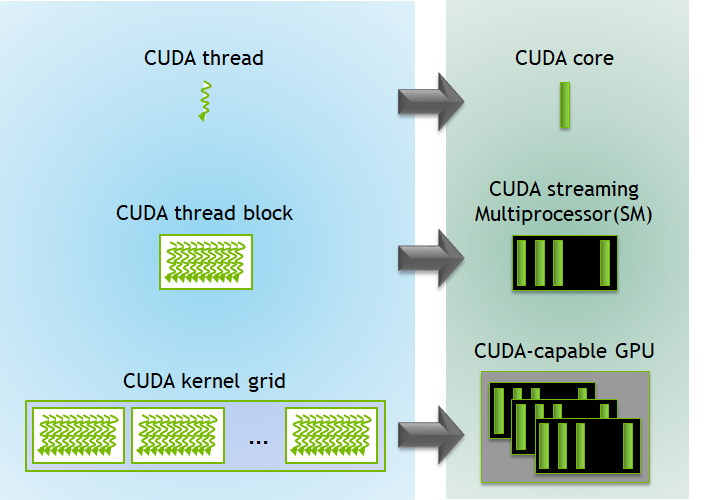
\includegraphics[width=0.7\linewidth]{figs/nvidia-cuda-model}
	\caption{Simplified overview of the CUDA programming model \cite{CUDARefresher2023}}
	\label{fig:nvidia-cuda-model}
\end{figure}



% TODO talk about how one may use a kernel for a simple task - E.g. addition of two vectors.

\section{CUDA-sDBSCAN}
CUDA-sDBSCAN is an accelerated implementation of sDBSCAN using GPU hardware. It has the same underlying steps as the original CPU implemented sDBSCAN, except operations are transferred to the GPU when necessary. CUDA-sDBSCAN retains the same parameters as sDBSCAN, and adds a few hyper-parameters to account for the use of a GPU. We break down CUDA-sDBSCAN along similiar lines to sDBSCAN, there is preprocessing, identification of key points and clustering. C

\subsection{Preprocessing}
The process of finding the closest/furthest $k$ random vectors to each query point $\bq$, and the closest/furthest $m$ data points can be easily parallelised using the power of a GPU. sDBSCAN's preprocessing steps can be rewritten for the GPU using a few key steps; these are described below.

\subsubsection{Performing Random Projections}
The projections between each dataset point $\bx_i$ and a given random vector $\br_j$ can be easily parallelised using a large matrix multiplication. This matrix multiplication can be easily paraellized using GPU hardware.

\begin{enumerate}
    \item First, create a matrix $\bR \in \mathbb{R}^{d \times D}$ containing $D$ random vectors, the shape of $R$ means that $D$ random vectors of length $d$ are stored \textit{column-wise} within it.
    \item Re-express the set of data points $X$ into a matrix $\bX \in \mathbb{R}^{n \times d}$, the shape of $\bX$ means that the $n$ dataset points of length $d$ are stored \textit{row-wise} within it.
\end{enumerate}

Now given the matrices $\bR$ and $\bX$, simply calculate the matrix product $\bP=\bX\bR$. A given entry $\bP_{ij}$ is then the projection of the data point $\bx_i$ onto the random vector $\br_j$.

\subsubsection{Ranking $k$ and $m$ closest/furthest vectors}
While the original CPU implementation of sDBSCAN relied on a priority queue approach with ranking the $k$ closest/furthest random vectors to each dataset point (and vice-versa for the top $m$ closest/furthest data points to each random vector), using the power of a GPU, we can make this process much simpler. Consequently, we simply \textit{sort} the projections matrix $P$ first along the rows, then along the columns to complete this process. Since a GPU can sort individual rows or columns in parallel, this is a relatively trivial and quick step.


\section{Experiment}

\section{Conclusion}

\bibliographystyle{plain}
\bibliography{refs, refs-related}

\end{document}
